\cleardoublepage

\chapter{Methods and problems in dream research}
\label{sec:dream-research}

\cleanchapterquote{La science du rêve occupe, sous ces rapports, une situation intermédiaire entre l’histoire et la biologie. Elle est une science d’observation en ce que l’observation y joue le rôle essentiel, mais elle est une science historique en ce sens que le rêve écoulé ne peut jamais être reproduit et qu’il est étudié, non directement, mais par l’intermédiaire du souvenir.}{Yves Delage}{Le rêve. Etude psychologique, philosophique et littéraire. 1920}

\section{Dreams}
\label{sec:dream-research:dreams}

\subsection{Definition}
\label{sec:dream-research:dreams:definition}

According to the Cambridge Dictionary, a dream is a \q{series of events or images that happen in the mind when one is sleeping}. This vague definition illustrates quite clearly how little we know about dreams, despite more than a century of experimental research and millennia of religious and philosophical speculation on their nature and meaning. The main reason for this lack of a clear and consensual definition (\cite{pagel_definitions_2001}) is that dreaming is \q{a phenomenon that we can solely observe during its absence} \footnote{Free translation from French: \q{Le rêve est le phénomène que nous n'observons que pendant son absence.}}(Paul Valery, Analecta, 1926).  Indeed, we still do not know precisely when dreaming occurs during sleep, and the dreamer alone is witness to his or her dream. For that reason, the scientific study of dreaming relies critically on the introspective recall of the dreamer, or \q{retrospection} \citep{schwartz_dreaming:_2005}.

\subsection{Scientific perspective}
\label{sec:dream-research:dreams:science}

Therefore, a more scientific definition of dreaming was proposed by \citet{guenole_a_2009} who wrote that \q{dreaming is a mental experience during sleep, which can be remembered and reported at wake}. He further distinguished three successive and intertwined forms of the dreaming phenomenon. The primordial state is the dream-experience that happens during sleep, and of which very little is known because the dreamer has no means to communicate in real-time his or her oneiric experiences to the external world. With the notable exception of lucid dreaming, the dream-experience is unobservable to the waking consciousness, be it that of an external observer, but also that of the dreamer him- or herself. The second form is the memory of the dream-experience as we recall it after awakening. Importantly, the dream recall occur in a consciousness state different from the one in which the dream was experienced. As a memory object, dream recall is therefore likely to be influenced by several mechanisms such as forgetting, reconstruction and censorships (\cite{schwartz_sleep_2002, schwartz_dreaming:_2005}). The third and last form is the dream report, obtained after transcription of the dream recall using words or pictures. It can be subject to verbal description difficulties and censorships The dream report is the only one that can actually be communicated to others and therefore the only one eligible to empirical investigation. As a consequence, most of the dream research has focused on dream reports.

\begin{figure}[htb]
	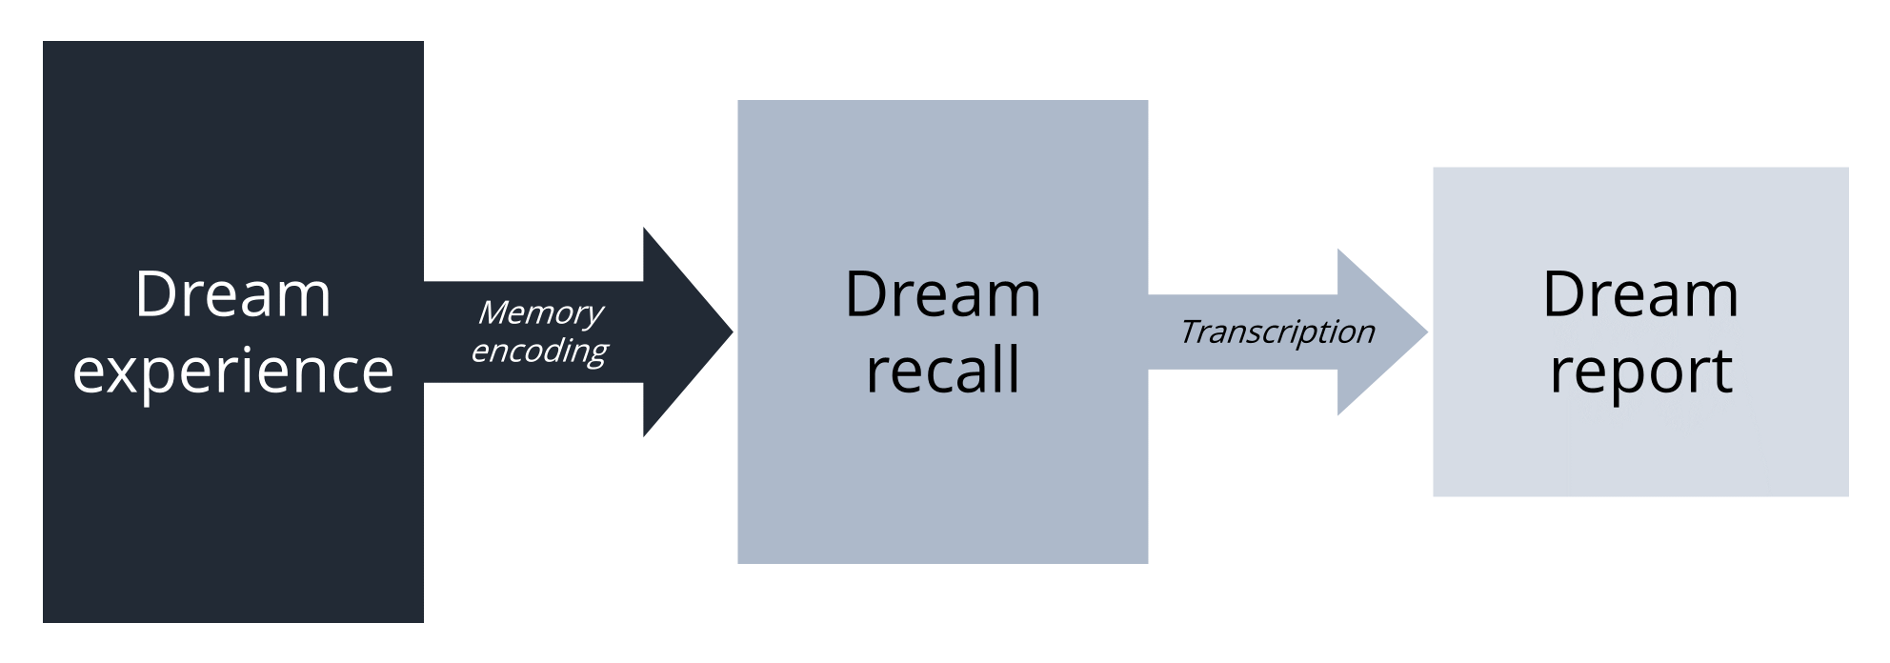
\includegraphics[width=\textwidth]{Fig/Intro/Intro_Guenole/Intro_Guenole.png}
	\caption[Guénolé's model of dreaming]{The three successive and intertwined forms of the dreaming phenomenon according to Guenolé's model. Adapted from \citet{guenole_a_2009}}
	\label{fig:intro:guenole}
\end{figure}

Because of this elusiveness of dreams and the constraints inherent to the scientific study of dreaming, it still remains one of the great mystery of the human cognition. Several questions on its nature and meaning are still not answered: do we dream every night? For how long? Why do we sometimes recall our dreams and sometimes not? Do dream reports obtained after awakening accurately convey subjective sleep experiences? What is, or what are, the function(s) of dreaming? What are the neurophysiological correlates of dreaming? The aim of the present thesis is to offer a modest contribution to the ongoing effort to solve these questions.

\section{Sleep}
\label{sec:dream-research:sleep}

As Schopenhauer rightly noticed, \q{the characteristic of dream is the condition of sleep peculiar to it}. Therefore, we cannot go any further in our study of dreaming without first defining the sleeping state and its physiology. Sleep is a normal physiological and periodic state characterized by vigilance suspension, which generally occurs during night time in humans. Sleep is a vital need that allows restoration of the immune, nervous, skeletal and muscular systems, leading some authors to postulate that \q{sleep is the price we pay for being alive} \citep{tononi_sleep_2014}. Long regarded as an idle state, it is becoming increasingly evident that sleep is \q{first and foremost a brain process} \citep{hirshkowitz_normal_2004} in which the brain is \q{hard at work and helps makes something of the world}, to borrow the words of Heraclitus’s famous aphorism (for an exhaustive review of the cognitive processes occurring during sleep, \citealt[see][]{andrillon_sleeping_2016}).

\subsection{Sleep stages}
\label{sec:dream-research:sleep:stages}

The invention of electro-encephalography (EEG) by Hans Berger in 1928 has paved the way for the scientific study of sleep. It was indeed soon after that discovery that Alfred Loomis first described a global slowing down of the brain rhythm during sleep, associated with the apparition of several grapho-elements such as K-complexes. Since then, sleep researchers have used EEG to monitor brain waves, electrooculography (EOG) to monitor eye movements and electromyography (EMG) to measure skeletal muscle activity. The simultaneous collection of these measurements is called polysomnography (PSG) and provides sufficient information to identify sleep stages according to standard international established guidelines. PSG is the gold standard in modern sleep science and is used in both clinical and research settings.

A first set of rules were published by Rechtschaffen and Kales (R\&K) in \citeyear{kales_manual_1968} and proposed to divide sleep into 5 stages with distinct electrophysiological properties, named rapid-eye movement (REM) and non-REM (NREM) stages 1, 2, 3, 4. This nomenclature was updated in 2007 by the American Academy of Sleep Medicine \citep{iber_aasm_2007} and sleep stage 3 and 4 have been merged into stage N3. Below are summarized EEG-EOG-EMG characteristics for wakefulness and the different sleep stages in healthy individuals (\citealp{hirshkowitz_normal_2004}; see also Figure \ref{fig:intro:sleep_stage}).

\paragraph{Wakefulness}
Before diving into sleep, we first need to define the state of wakefulness. Eyes-closed quiet wakefulness is accompanied by an EEG rhythm predominantly in the alpha range (8 - 12 Hz). Opening the eyes or engaging in a significant mental task (for example mental calculation) reduces or blocks the alpha activity. Fairly high muscle activity can be present and slow or rapid eye movements may occur.

\paragraph{N1 sleep}
Stage N1 corresponds to the transitional period between wakefulness and sleep. The brain rhythm progressively decreases from alpha to theta (5 – 7 Hz), and the EOG is characterized by slow, rolling eye movements. N1 sleep represents approximatively 5\% of a normal night of sleep.

\paragraph{N2 sleep}
Each night, we spend more than half the night’s sleep in N2 sleep. The EEG activity during this stage is characterized by a predominance of theta waves, recurrently interrupted by two grapho-elements, the spindles and K-complexes, which are the landmarks of this sleep stage. K-complexes are defined as sharp negative waves followed by a positive component, prominent over frontal scalp electrodes and lasting more than 0.5 seconds. Spindles refer to burst of 12 to 14 Hz waves predominant over central scalp electrodes and lasting between 0.5 and 2 seconds. Beyond that, N2 sleep is characterized by an absence of eye movements as well as decreased muscle tone and brain metabolism.

\paragraph{N3 sleep}
N3 sleep, also referred to as deep sleep or slow-wave sleep, is the deepest sleep stage. It is characterized by a predominance (> 20\% of the epoch) of high amplitude (> 75 µV) delta waves (0.5 – 4 Hz). Eye motility, muscle tone and brain metabolism are even more decreased than in N2 sleep. N3 sleep represents approximatively 20\% of a normal night of sleep.

\paragraph{REM sleep}
As its name suggests, rapid eye movements (REM) sleep is characterized by rapid eye movements easily observable on the EOG channels. They consist of conjugate, irregular and sharply peaked eye movements, similar to some extent to those exhibited during wakefulness. Another fundamental aspect of REM sleep is its muscle atonia, as revealed by a low EMG activity. However, some transient muscle activity or muscle twitching (MTs) can also be observed. These short irregular bursts of EMG activity are superimposed on the background of low EMG activity. Brain metabolism is similar to that of wakefulness, and the EEG is marked by mixed low-amplitude waves predominantly in the theta band (saw-tooth waves), as well as a complete absence of delta rhythms. Other physiologic activities accompany REM sleep including middle ear muscle activity, periorbital integrated potentials, and sleep-related erections. REM sleep constitutes approximatively 20\% of a normal night of sleep.

% \begin{figure}[htb]
% 	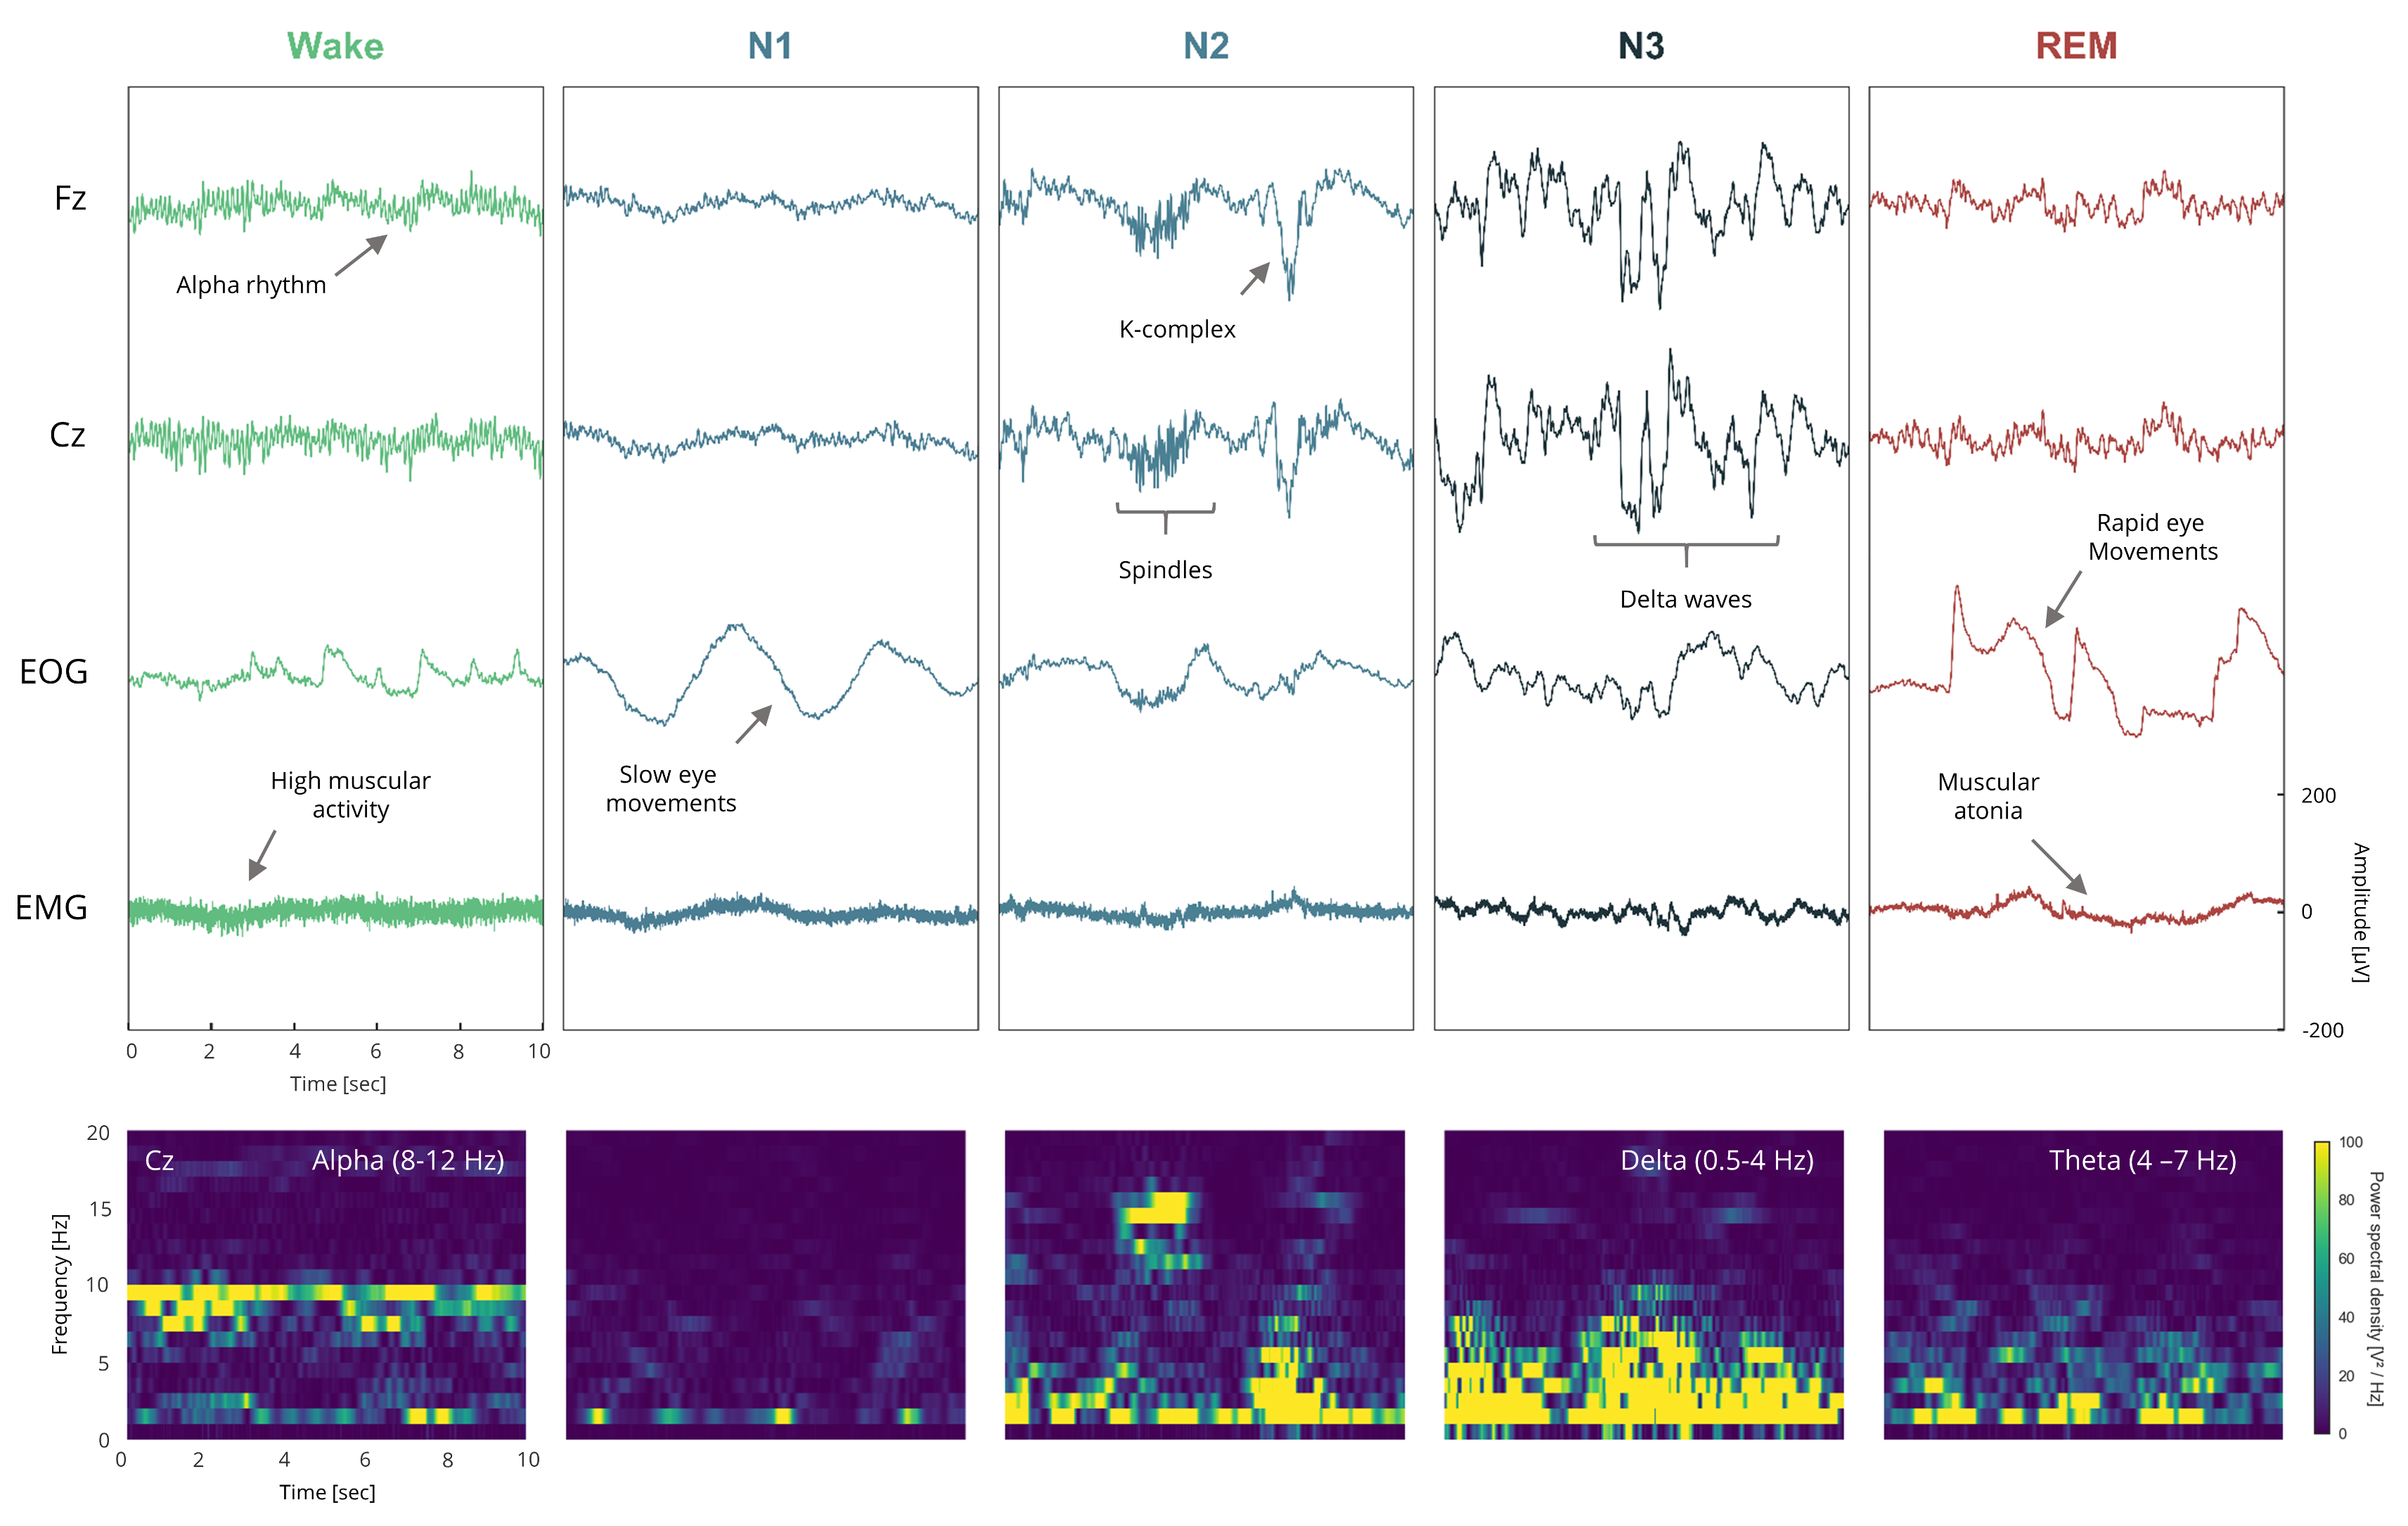
\includegraphics[width=\textwidth]{Fig/Intro/Intro_Sleep_Stages_PSD/Intro_Sleep_Stages_PSD.png}
% 	\caption[Polysomnographic recordings across sleep and wakefulness]{Polysomnographic recordings across sleep and wakefulness. Top: Scalp EEG, EOG and EMG performed in one healthy young adult during wakefulness, N1, N2, N3 and REM sleep. The main features of each vigilance state are described. Bottom: Spectral properties of each stage obtained by computing the spectrogram of the Cz EEG signal atop.}
% 	\label{fig:intro:sleep_stage}
% \end{figure}

\begin{sidewaysfigure}[htbp]
	\centering
	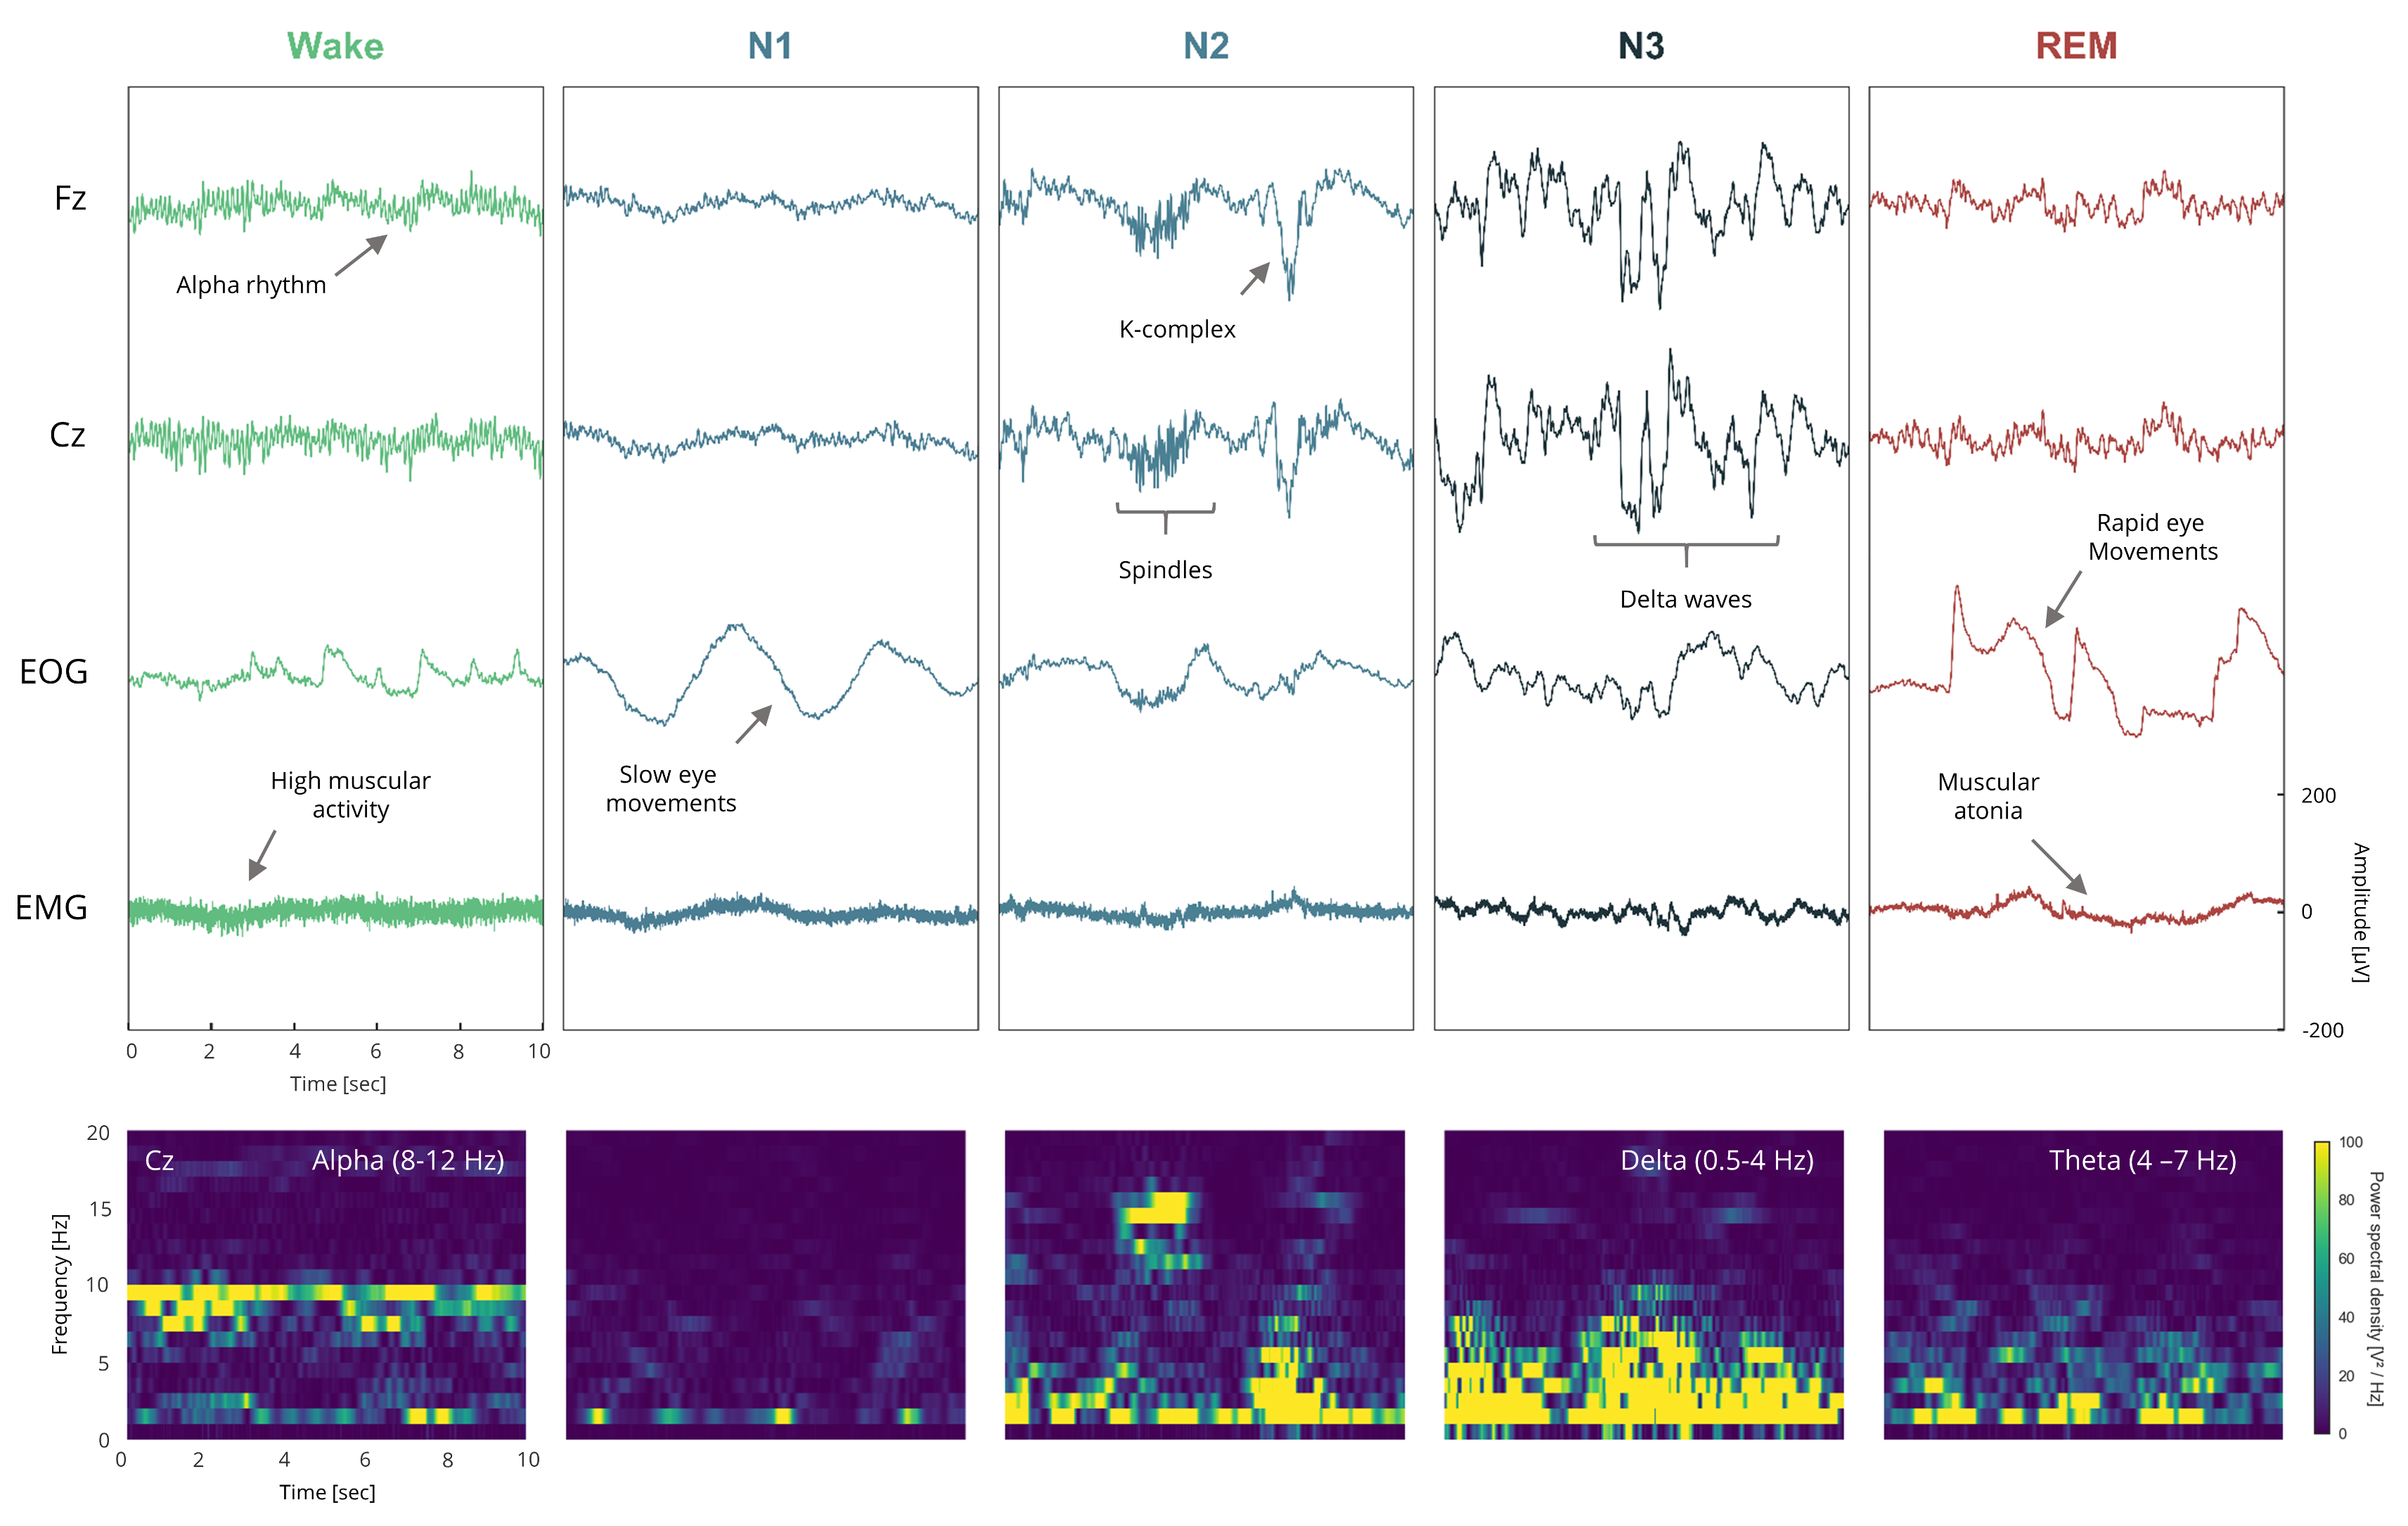
\includegraphics[width=\linewidth, height=0.8\textheight, keepaspectratio]{Fig/Intro/Intro_Sleep_Stages_PSD/Intro_Sleep_Stages_PSD.png}
	\captionsetup{width=0.9\textheight}
	\caption[Polysomnographic recordings across sleep and wakefulness]{Polysomnographic recordings across sleep and wakefulness. Top: Scalp EEG, EOG and EMG performed in one healthy young adult during wakefulness, N1, N2, N3 and REM sleep. The main features of each vigilance state are described. Bottom: Spectral properties of each stage obtained by computing the spectrogram of the Cz EEG signal atop.}
	\label{fig:intro:sleep_stage}
\end{sidewaysfigure}

\subsection{Sleep architecture}
\label{sec:dream-research:sleep:architecture}

Modern research has revealed that sleep is not a unitary, single block, but rather a cyclical succession of different brain states, which are all associated with specific functional roles. A normal night of sleep consists of a repetition of four or five 90 to 110 minutes long cycles in which sleep stages tend to follow each other in a particular order. The sleep cycle properties evolve with each cycle re-occurrence. Sleep staging is generally done visually by inspecting consecutive polysomnographic segments of 30 seconds. It results in a hypnogram which represents the succession of sleep stages across time (Figure 3). In his overview of the human sleep, \citet{hirshkowitz_normal_2004} described five generalizations about normal sleep architecture:

\begin{my_list_num}
    \item Sleep is entered through non-REM sleep
    \item Non-REM and REM sleep alternate approximately every 90 to 120 minutes
	\item N3 sleep predominates in the first third of the night
	\item REM sleep predominates in the last half of the night
	\item REM sleep occurs in four to six discrete episodes each night with episodes generally lengthening as sleep period progresses
\end{my_list_num}

\vspace{10mm}

\begin{figure}[htb]
	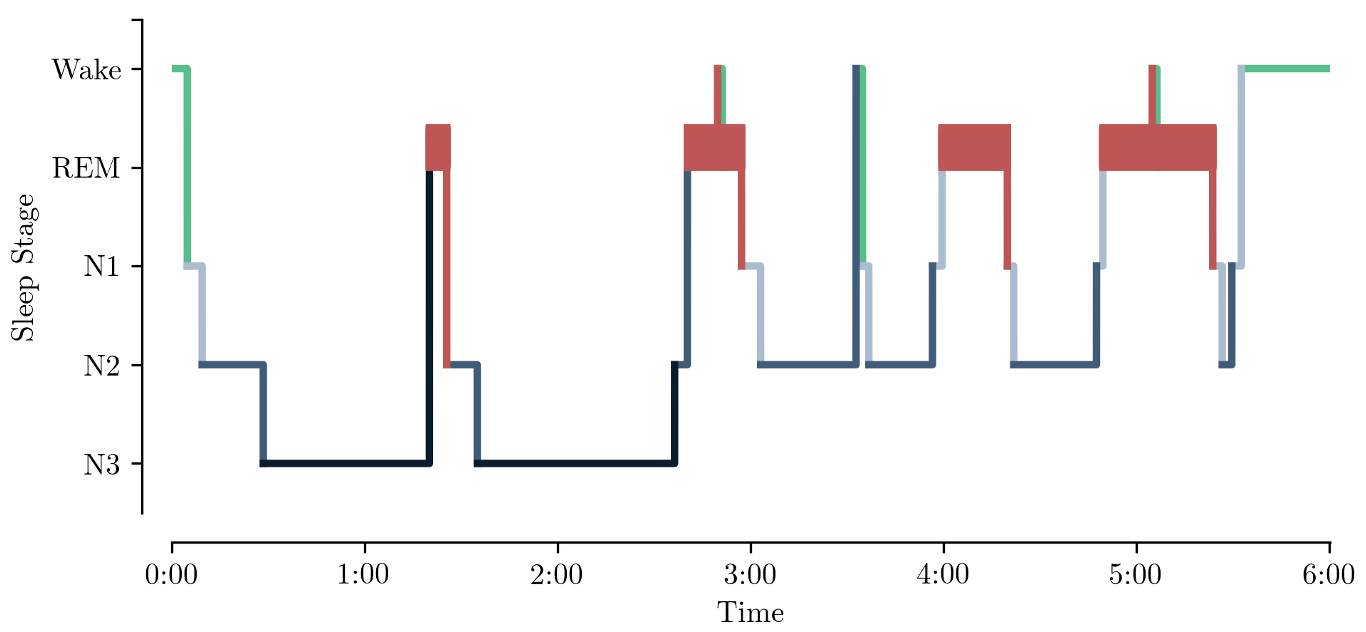
\includegraphics[width=\textwidth]{Fig/Intro/Intro_Hypnogram/Intro_Hypnogram.png}
	\caption[Example hypnogram of a healthy adult]{Example hypnogram of a healthy adult. The hypnogram is a graph which represents the stages of sleep as a function of time.One can easily recognize the succession of sleep cycles and especially the alternation of NREM (blue gradient) and REM sleep (red). Note that the hypnogram graph was generated directly as it is from the sleep software presented in the experimental results section.}
	\label{fig:intro:hypno}
\end{figure}

% \subsection{Neurochemistry of REM and NREM sleep}
% \label{sec:dream-research:sleep:neurochemistry}
%
% The brain undergoes dramatic alterations in neurochemistry as it passes through the different sleep stages. NREM sleep is marked by a strong deactivation of subcortical cholinergic systems, and to some extent, a relative deactivation of aminergic systems (e.g. histamine, serotonin, and norepinephrine) compared to wakefulness. By contrast, REM sleep is characterized most notably by an abundance of the neurotransmitter acetylcholine, combined with a nearly complete absence of aminergic modulation.

\section{Link between dreaming and sleep stages}
\label{sec:dream-research:link}

\subsection{Goblot's hypothesis}
\label{sec:dream-research:link:goblot}

\q{The dream, some said, is the thought of sleep. Has someone ever questioned the accuracy of this formula? I think it should be amended and rather say: \emph{the dream that one remembers is the thought of awakening}}. \footnote{Free translation from French: \q{Le rêve, à t-on dit, est la pensée du sommeil. A-t-on jamais songé à mettre en doute l'exactitude de cette formule? Je pense qu'il convient de la modifier, et de dire : \emph{Le rêve dont on se souvient est la pensée du réveil}}} It is with these words that \citet{goblot_souvenir_1896} start his article \q{Le souvenir des rêves}, which postulates that dreaming does not occur during sleep but only at the moment of awakening.

While this claim has enthralled several philosophers and neurobiologists in the twentieth century, numerous and robust experimental data in sleep psychophysiology clearly demonstrated that dreaming does take place during sleep (reviewed in \citealp{guenole_reve_2010}). Perhaps one of the most significant evidence against this claim is the scientifically-verified existence of lucid dreaming during REM sleep (i.e. the ability to become self aware of dreaming during a dream, see section \ref{sec:dream-research:attempts:ba-lucid}; \citealp{laberge_exploring_1991, dresler_neural_2012}), which clearly shows that dreaming (albeit a somewhat modified form of it) does occur during sleep. Other proofs against this hypothesis come from the study of parasomnias, such as sleep-talking or REM sleep behavior disorder, during which the dream content is (sometimes) correlated to the sleep behavior \citep{ellman_mind_1991, schenck_rem_2002, leclair-visonneau_eyes_2010}. Further evidence can be found by looking at the incorporation of non-awakening stimulations in subsequent dream reports. Using such a paradigm, \citet{dement_relation_1958} found that tactile (water) stimulation was incorporated 42\% of the time, and reported that the subjective time interval between the incorporation of the stimulus and the awakening was comparable within the dream and in waking-life.

\subsection{The REM sleep hypothesis of dreaming}
\label{sec:dream-research:link:rem-sleep}

In the early fifties, Nathaniel Kleitman and his doctoral student Eugene Aserinsky, discovered in humans the existence of periods of sleep with an EEG similar to wakefulness (low voltage and fast frequencies), rapid eye movements and neurovegetative responses \citep{aserinsky_regularly_1953}. This discovery had a strong and persistent impact on dream and sleep research. The authors have indeed proposed that the rapid eye movements corresponded to the scanning of dream images. They reached this conclusion by comparing the proportion of dream reports obtained upon awakening in periods of eye motility and outside these periods, respectively 75\% and 11\% in their 1953’s study, and 80\% and 7\% in their 1957's study \citep{dement_relation_1957}. They concluded that their newly-discovered REM sleep stage was the neurophysiological basis of dreaming. A few years later, the French neurophysiologist Michel Jouvet, who had started working on sleep in cats, found that REM sleep was associated with muscular atonia \citep{jouvet_sur_1959}, a finding that was soon after replicated in humans \citep{berger_tonus_1961}. Pursuing his research on REM sleep, or \q{paradoxical sleep} as he named it, Jouvet had the idea to suppress the muscular atonia by injuring the brain stem of cats. To his astonishment, he found that the injured cats were performing, only during REM sleep, complex motor sequences, that he named \q{oneiric behavior} \citep{sastre_comportement_1979}. For him and the scientific community at the time, it was clear that these motors sequences were directly related to the cat's dreams, and this experiment provided a significant evidence in favor of the REM sleep hypothesis of dreaming.

However, even though equating dreaming with REM sleep provided a useful way to scientifically explore dreaming, it soon became apparent that dreaming was in fact not exclusively present during REM sleep but also during all the other sleep stages. Few years after the initial discovery of REM sleep, several researchers reported a much higher proportion of dream report in non-REM sleep than what was expected based on the findings of the Kleitman’s team \citep{goodenough_comparison_1959, foulkes_dream_1962}. Comparing the recall rate of people who never remembered their dreams with people who frequently recalled them, Goodenough and colleagues found respectively 34\% and 54\% of dream reports outside of REM sleep. The recall rate went up to 54\% in Foulkes’s study which comprised 200 awakenings. Since then, numerous studies have replicated the finding of mentation outside of REM sleep \citep{nielsen_review_2000}, even in the periods of non-REM sleep located before the first nocturnal episode of REM sleep \citep{noreika_early-night_2009}. As a counterpoint, it has become apparent that a significant proportion (~15\%) of REM sleep awakenings were not followed by a dream report. Taken together, these results demonstrate that REM sleep is not the neurophysiological substrate of dreaming. It is noteworthy that this hypothesis is still predominant in the public mind, and to some extent in the scientific community. As Schwartz and colleagues aptly pointed out, \q{REM sleep is not a necessary, but a facilitating condition for dreaming to occur. Conversely, there is little doubt that dreaming was a necessary condition for REM sleep to become famous} \citep{schwartz_dreaming:_2005}.

\subsection{The fore-brain hypothesis of dreaming}
\label{sec:dream-research:link:solms}

Fervent supporter of the REM sleep hypothesis of dreaming, Allan Hobson argued that dreaming was generated by random neural signals originating within the brainstem during REM sleep (see section \ref{sec:dream-func:modern:nofunc}, \citealp{hobson_dream_1998}). His theory was the dominant view for several decades until Mark Solms refuted it using neuropsychological evidences. He examined 361 neurological patients and asked them in detail about their dreaming \cite{solms_neuropsychology_1997}. He found that out of 26 case reports of REM sleep loss or alteration following a lesion in the brainstem (Pons area), 25 were not associated with subsequent alterations in dream reporting. By contrast, he reported that in most cases global cessation of dreaming (a condition referred to as the Charcot-Wilbrand syndrome) followed lesions in or near the temporo-parietal junction (TPJ) and the medial prefrontal cortex (MPFC; see Figure \ref{fig:intro:lesions}). Importantly, damage in these two regions were rarely associated with REM sleep disturbances. This double dissociation provides a clear argument that not only dreaming can occur outside of REM sleep, but it is also not dependent of the brainstem generators of REM sleep. This led Solms to put forward the fore-brain hypothesis of dreaming, which proposes that dreaming is controlled through forebrain mechanisms involving at least TPJ and MPFC.

\begin{figure}[htb]
	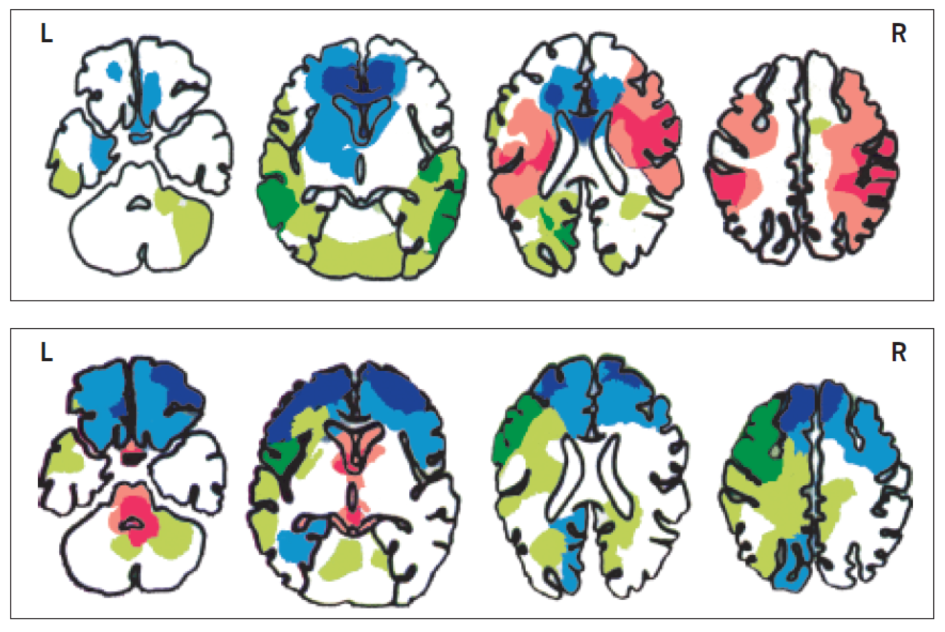
\includegraphics[width=\textwidth]{Fig/Intro/Intro_Lesions/Intro_Lesions.png}
	\caption[Lesion maps associated with cessation vs preservation of dreaming]{Lesion maps associated with cessation vs preservation of dreaming. Top: Global cessation of dreaming was found following parietal lobe lesions (6 cases, inferior lobule and supramarginal gyrus; red), medial frontal lesions (9 cases; blue), and posterior lesions (8 cases; green). Bottom: Preserved dreaming was found following left hemispheric and frontal convexity lesions (15 cases; green), bifrontal lesions (14 cases; blue), and brainstem lesions (17 cases; red). Reproduced from \citet{schwartz_dreaming:_2005}}
	\label{fig:intro:lesions}
\end{figure}

\subsection{A continuum of mentation during sleep}
\label{sec:dream-research:link:continuum}

Based on Solms’s findings, some authors have postulated that instead of relying on REM sleep mechanisms, dreaming might be best described along a \q{continuum} of mentation during sleep, ranging from the hypnagogic reveries typical of sleep onset to florid and vivid dreamlike experiences typical during REM sleep \citep{schwartz_dreaming:_2005}. A brief description of this continuum of mental activities during sleep is reported in Table \ref{tab:intro:continuum}.

\begin{table}[htb]
	\caption[A continuum of sleep mentation]{A brief description of sleep mentation in their typical order of placement during the sleep cycle. Modified from \citet{de_koninck_sleep_2012}}
	\label{tab:intro:continuum}
	\begin{tabularx}{\textwidth}{XXX}
	\toprule
	Name                  		   & Description                                                                          		   & Sleep stage                         			\\ \midrule
	Hypnagogic reverie             & Simple images                                                                                 & Sleep onset mentation (N1 or early N2 sleep) 	\\
	Reflections                    & Thoughts with no hallucinatory content                                                        & N2 sleep                                     	\\
	Vivid dreams                   & Vivid imagery and sequences, presence of characters, interactions and emotions                & REM and NREM sleep                           	\\
	Lucid dreams                   & The dreamer is conscious of dreaming and can sometimes controls the dream scenario            & REM sleep                                    	\\
	Nightmares and bad dreams 	   & Unpleasant and highly anxiogenic dream. The content of nightmare actually awakens the dreamer & REM sleep                                    	\\
	Hypnopompic reverie            & Characterized by elaborate imagery                                                            & Sleep offset mentation (REM or NREM sleep)   	\\ \bottomrule
	\end{tabularx}
\end{table}


\section{Attempts to study the cerebral correlates of dreaming}
\label{sec:dream-research:attempts}

Thanks to the recent advances in neuroimaging techniques, we have the means to measure, with unprecedented spatial and temporal accuracy, what is happening in the brain at a specific moment in time (see Methods section). Yet, since it is now well-accepted that dreaming can occur in all sleep stages, and because dream consciousness is only accessible via report rather than direct observation, it is therefore impossible to be sure that dreaming is happening at a specific time point during sleep. This conceptual issue has not prevented sleep and dream researchers to attempt to identify the cerebral correlates of dreaming. The main methods and findings are summarized in the following paragraphs.

\subsection{Brain activity during REM sleep}
\label{sec:dream-research:attempts:ba-rem}

On the basis of the REM sleep hypothesis of dreaming, which was predominant during the nineties, researchers used functional neuroimaging techniques such as positron emission tomography (PET) to investigate the brain activity during REM sleep. They reported that, despite strong similarities between the wake and REM sleep electrophysiological scalp signals, the brain metabolism in these two vigilance states was disparate \citep{maquet_functional_1996, braun_regional_1997}. Among the most notable findings, the regional cerebral blood flow (rCBF) was decreased in several brain regions including the dorsolateral prefrontal cortex (DLPFC), and was increased in other regions (occipital, temporal, and superior parietal cortices, hippocampal formation, anterior cingulate and the pons). Following these works, researchers postulated that these changes in the brain functional organization could explain the phenomenological characteristics of dream reports \citep{hobson_dreaming_2000, nir_dreaming_2010}. For instance, increased occipital cortex activity during REM sleep could explain the clear predominance of visual modality in dream reports, a phenomenon that Vincent van Gogh had already noticed when he wrote: \q{I often think that the night is more alive and more richly colored than the day} (Vincent van Gogh, 1888). Second, the increased activity during REM sleep in the hippocampal formation, a region well-known for its role in memory encoding and retrieval, could account for the presence of known images and characters in dreams. Finally, the decreased activity in the dorsolateral prefrontal cortex, a region involved in executive function, cognitive control and working memory, could account for the lack of consistency, voluntary control and logical reasoning over the dream story. This is consistent with studies on lucid dreaming which showed a partial reactivation of this area in lucid dreams compared to non-lucid dreams. We will return to these correspondences between the phenomenology of dreams and brain activity in section \ref{sec:dream-research:attempts:dmn}.

\subsection{Brain activity during lucid dreaming}
\label{sec:dream-research:attempts:ba-lucid}

Long considered as a fantasy, lucid dreaming - the ability to become self-aware of dreaming during a dream, and in some cases, to control the dream scenario – has recently gained considerable interest among researchers and the public. The scientific study of lucid dreaming started in the nineteenth century when Hervey de Saint Denys, a learned oneirologist, published his landmark book \q{Dreams and the Ways to Direct Them: Practical Observations}, in which he described his own lucid dream experiences. More than a century later, more objective methods such as EEG and functional magnetic resonance imaging (fMRI) have become the technique of choice for understanding lucid dreams. Using a pre-determined ocular signal, Dresler was remarkably able to measure, in real-time, the brain activity during lucid REM sleep and non-lucid REM sleep (though only one subject out of four had lucid dreams of sufficient length; \citealp{dresler_neural_2012}). Lucid REM sleep was associated with a reactivation of areas that are normally deactivated during REM sleep, such as bilateral precuneous, parietal lobules and prefrontal and occipito-temporal cortices. Phenomenologically, these regions are either involved in self-awareness and executive functions, and their reactivation during lucid dreaming could account for the resurgence of a certain level of self-awareness and voluntary control. Even more recently, Voss was able to induce self-reflective awareness during dream using fronto-temporal transcranial alternating current stimulation \citep{voss_induction_2014}. They reported that lucid dreams were most prominent during stimulation in the lower gamma band (58\% of lucid dreams following a stimulation at 25 Hz and 77\% of lucid dreams following a stimulation at 40 Hz). However, the lucidity was not assessed directly by the dreamer but assumed a posteriori if the subjects reported elevated ratings on a lucidity scale. In conclusion, lucid dreaming provides an appealing and elegant way to study, in real time, the cerebral correlates of dreaming. Yet, the inherent problem with this method lies precisely in the fact that lucid dreams are, by nature, different from non-lucid dreams. As exciting as the results are, it would be however difficult to generalize them to the research on non-lucid dreams.

\subsection{Brain activity in the minutes preceding a dream report}
\label{sec:dream-research:attempts:ba-pre}

Another line of research consists in comparing the pre-awakening sleep EEG spectral power associated with the presence or absence of a dream report. This paradigm has been used in several studies over the years, the findings of which are summarized in Table \ref{tab:intro:ba-pre}.

\citet{esposito_reduced_2004} reported that in both REM and N2 sleep, dream recall was associated with a lower alpha and delta power in the 3 minutes preceding awakening. According to the authors, the alpha effect may reflect increased cognitive elaboration and visual imagery as well as increased attention and memory processes. A few years later, \citet{marzano_recalling_2011} found that dream recall after morning awakening from REM sleep was associated with a higher frontal 5–7 Hz (theta) activity in the 5 minutes preceding awakening. In N2 sleep, dream recall was associated with a decrease in alpha power, an observation consistent with Esposito’s results. The same year, another study reported a lower delta power for the dream recall condition following awakening from N2 sleep, and a higher alpha and beta power in occipital derivations for REM sleep \citep{chellappa_cortical_2011}. Finally, a recent study reported that in both N2 and REM sleep, dream recall was associated with local decreases in delta power in posterior cortical regions in the 2 minutes preceding awakening \citep{siclari_neural_2017}. The authors were able to predict whether an individual reported dreaming or the absence of dream experiences after awakening from N2 sleep by monitoring this posterior ‘hot zone’ in real time.

In sum, the results from these studies are heterogeneous and sometimes contradictory. Moreover, despite this paradigm may seem attractive at first, there are two major issues with this methodology. First, we can never be sure whether the dream actually took place in the minutes just before awakening or several tens of minutes before. Second, as we already pointed out, it is impossible to know for sure whether the failure to recall a dream actually means that the sleeper was not dreaming, or rather that the sleeper was dreaming but did not remember it.

\mathversion{bold}
\begin{table}[!htb]
	\caption[Pre-awakening EEG spectral power associated with the presence of a dream report.]{\textbf{Review of the studies that investigated the pre-awakening sleep EEG spectral power associated with the presence or absence of a dream report.} {\color[HTML]{FE0000}$\nearrow$} The EEG spectral power is increased in this frequency band when subjects recalled a dream compared to when they did not recall one. {{\color[HTML]{3166FF} $\searrow$}} The EEG spectral power is decreased in this frequency band when subjects recalled a dream compared to when they did not recall one. = There is no EEG spectral power difference between the two conditions. * Higher occipital alpha, decreased frontal alpha. N = number of participants.}
	\label{tab:intro:ba-pre}
    \resizebox{\textwidth}{!}{%
    \begin{tabularx}{\textwidth}{Xlllll}
    \toprule
	\textbf{Study}                     	& \textbf{N} 	& $\delta$ (0.5-4Hz)     			& $\theta$ (4-7Hz)      			& $\alpha$ (8-12Hz)        												& $\beta$ (\textgreater13Hz) \\
	\midrule
	\textbf{\textit{REM sleep}}  & & & & & \\
	\citealp{moffitt_individual_1982}   & 8          	& =                        			& =                        			& =                          											& =                               		\\
	\citealp{lehmann_dream_1981}        & -       	    & {\color[HTML]{3166FF} $\searrow$} & {\color[HTML]{3166FF} $\searrow$} & {\color[HTML]{3166FF} $\searrow$}   									& =                               		\\
	\citealp{wollman_cortical_1987}     & 30         	& =                        			& =                        			& =                          											& =                               		\\
	\citealp{rochlen_eeg_1998}          & 17         	& =                        			& =                        			& =                          											& {\color[HTML]{FE0000} $\nearrow$}     \\
	\citealp{germain_fast_1999}         & 41         	& =                        			& =                        			& {\color[HTML]{FE0000} $\nearrow$}   									& {\color[HTML]{FE0000} $\nearrow$}     \\
	\citealp{takeuchi_eeg_2003}         & 8          	& =                        			& =                        			& {\color[HTML]{3166FF} $\searrow$}   									& =                               		\\
	\citealp{esposito_reduced_2004}     & 11         	& {\color[HTML]{3166FF} $\searrow$} & =                        			& {\color[HTML]{3166FF} $\searrow$}   									& =                               		\\
	\citealp{marzano_recalling_2011}    & 30         	& =                        			& {\color[HTML]{FE0000} $\nearrow$} & =                          											& =                               		\\
	\citealp{chellappa_cortical_2011}   & 17         	& =                        			& {\color[HTML]{000000} =} 			& {\color[HTML]{FE0000} $\nearrow$}{\color[HTML]{3166FF} $\searrow$}* 	& {\color[HTML]{FE0000} $\nearrow$}     \\
	\citealp{scarpelli_state-_2015}     & 6          	& =                        			& {\color[HTML]{FE0000} $\nearrow$} & =                          											& =                               		\\
	\citealp{siclari_neural_2017}       & 46         	& {\color[HTML]{3166FF} $\searrow$} & =                        			& =                          											& =                               		\\
	\smallskip
	\textbf{\textit{Non-REM sleep}} & & & & & \\
	\citealp{moffitt_individual_1982}   & 8          	& {\color[HTML]{3166FF} $\searrow$} & =                        			& =                          											& =                               		\\
	\citealp{williamson_spectral_1986}  & 6          	& =                        			& =                        			& =                          											& =                               		\\
	\citealp{morel_electrophysiological_1991} & 40      & =                        			& =                        			& =                          											& =                               		\\
	\citealp{takeuchi_eeg_2003}         & 8          	& =                        			& =                        			& {\color[HTML]{FE0000} $\nearrow$}   									& =                               		\\
	\citealp{wittmann_nrem_2004}        & 6          	& =                        			& =                        			& =                          											& =                               		\\
	\citealp{esposito_reduced_2004}     & 8          	& {\color[HTML]{3166FF} $\searrow$} & =                        			& {\color[HTML]{3166FF} $\searrow$}   									& =                               		\\
	\citealp{marzano_recalling_2011}    & 35         	& =                        			& =                        			& {\color[HTML]{3166FF} $\searrow$}   									& =                               		\\
	\citealp{chellappa_cortical_2011}   & 17         	& {\color[HTML]{3166FF} $\searrow$} & =                        			& =                         											& {\color[HTML]{3166FF} $\searrow$}     \\
	\citealp{scarpelli_predicting_2017} & 14         	& {\color[HTML]{3166FF} $\searrow$} & =                        			& =                          											& =                               		\\
	\citealp{siclari_neural_2017}       & 46         	& {\color[HTML]{3166FF} $\searrow$} & =                        			& =                          											& = 									\\
	\bottomrule
    \end{tabularx}%
    }
\end{table}
\mathversion{normal}

\subsection{Dreaming as a subsystem of the default mode network}
\label{sec:dream-research:attempts:dmn}

The past few years have witnessed the emergence of a new conceptual framework of dreaming, centered on the idea that dreaming is a unique form of mind-wandering, which cerebral correlates are a subsystem of the default mode network (DMN; see Methods section; \citealp{maquet_human_2005, domhoff_neural_2011, domhoff_dreaming_2015, christoff_mind-wandering_2016}). Based on the fact that dreaming and waking spontaneous thought share many features (i.e. predominance of the audiovisual modalities, centered on one’s current goals and concerns, draw heavily on semantic and episodic memory in constructing simulations and future plans, presence of a wide range of affect), some authors have postulated that dreaming is a \q{type of spontaneous thought that is highly unconstrained, hyper-associative and highly immersive} \citep{christoff_mind-wandering_2016}. Using the results of lesion and REM sleep neuroimaging studies, they argued that dreaming should be accompanied, at the neural level, by a strong recruitment of the default mode network medial temporal lobe (MTL)-centered subsystem and strong deactivations in frontoparietal control network regions (such as the DLPFC). Activation of the former areas could be related to the generation of spontaneous thoughts, during both wake and sleep, while the deactivation of the latter areas could explain the high volatility and variability of dream content over time.
